\section{The tent and the sine squared lemma}\label{yo:sec:tent}

Yoshida's basic vector is $\chi_0=(2a)^{-1/2}1_{[-a,a]}$, and $\chi_0*\widetilde{\chi_0}=(2a)^{-1}(2a-|y|)_+$. Put $x=2a$,
\[
\Delta_x(y)=(x-|y|)_+,\qquad D(x)=\mathcal Y(\Delta_x)=x\,\langle\chi_0,\chi_0\rangle,
\]
where $\chi_0$ is taken for $a=x/2$. So $\Delta_x$ is the tent of height $x$ on $[-x,x]$, and $D(x)$ is the single coefficient $\langle\chi_0,\chi_0\rangle$ of Yoshida's matrix multiplied by the length $x$ of the window.

\begin{proposition}\label{yo:prop:tent}
Let $k_x(w)=e^{-wx}+wx-1$ be the compensated exponential on the left of the sine squared lemma \eqref{eq:sin2}, and let $\gamma_\rho=-i(\rho-\frac12)$, which is complex for an off line zero.
\begin{itemize}
\item[(a)] For complex $w$ and real $t$,
\[
\begin{gathered}
\int_{\R}\Delta_x(y)e^{wy}\,dy=\frac{k_x(w)+k_x(-w)}{w^2}=\frac{4\sinh^2(wx/2)}{w^2},\\
\widehat{\Delta_x}(t)=\frac{4\sin^2(xt/2)}{t^2}\ge0 .
\end{gathered}
\]
\item[(b)] Unconditionally $D(x)=\sum_\rho4\sin^2(\gamma_\rho x/2)/\gamma_\rho^2$, the sum over all nontrivial zeros. Under RH, with the Thorin measure $U=\sum_{\gamma>0}\delta_{\gamma^2}$ of Proposition~\ref{prop:rigid},
\[
\begin{aligned}
D(x)&=8\int\frac{\sin^2(x\sqrt t/2)}{t}\,U(dt)\\
&=\frac{8\pi}x\int\frac{x\sin^2(x\sqrt t/2)}{\pi\sqrt t}\,\frac{U(dt)}{\sqrt t},
\end{aligned}
\]
so $D$ samples the Thorin density of the sine squared lemma \eqref{eq:sin2} at level $x$ on the Thorin atoms $t=\gamma^2$, with the weight $t^{-1/2}$.
\item[(c)] Unconditionally,
\[
D(x)=32\sinh^2\frac x4-x\log\pi-2\sum_{n\le e^x}\frac{\Lambda(n)}{\sqrt n}\log\frac{e^x}{n}+V_1(\Delta_x),
\]
\[
\begin{aligned}
V_1(\Delta_x)&=x-x\log x-(\gamma_E+\log2)x\\
&\quad-2\int_0^x\Bigl(\frac{e^{y/2}}{2\sinh y}-\frac1{2y}\Bigr)(x-y)\,dy,
\end{aligned}
\]
and the prime term is a Riesz mean of order one of $\Lambda(n)n^{-1/2}$.
\item[(d)] With $\psi$ the digamma function, $V_1(\Delta_x)$ is also the residue series
\[
V_1(\Delta_x)=x\,\psi(\tfrac14)+\tfrac12\psi'(\tfrac14)-2\sum_{k\ge0}\frac{e^{-(2k+1/2)x}}{(2k+\frac12)^2}.
\]
\end{itemize}
\end{proposition}

\begin{proof}
(a) Taylor's formula with integral remainder gives $k_x(w)=w^2\int_0^x(x-y)e^{-wy}dy$, so $\int\Delta_xe^{wy}dy=(k_x(w)+k_x(-w))/w^2$, and $k_x(w)+k_x(-w)=e^{wx}+e^{-wx}-2=4\sinh^2(wx/2)$; put $w=it$.

(b) Evaluate $\widehat{\Delta_x}$ at $\gamma_\rho$ and sum over the zeros; the series converges absolutely, since $|\sin^2(x\gamma_\rho/2)|\le\cosh^2(x/4)$ for $|\im\gamma_\rho|<\frac12$ and $\sum|\gamma_\rho|^{-2}<\infty$. Under RH group $\pm\gamma$, which gives $D(x)=2\sum_{\gamma>0}4\sin^2(\gamma x/2)/\gamma^2$.

(c) Insert $\Delta_x$ in \eqref{yo:EF}. By (a) at $w=\pm\frac12$ the first term is $2\cdot4\sinh^2(x/4)/(1/4)=32\sinh^2(x/4)$, the second is $-(\log\pi)\Delta_x(0)=-x\log\pi$, and $\Delta_x(\log n)+\Delta_x(-\log n)=2(x-\log n)_+$. For $V_1$ use the second form of \eqref{yo:V1}, with $\operatorname{Pf}(1/|y|)(\Delta_x)=2(x\log x-x)$ for all $x>0$, because $\int_{\epsilon<|y|<x}(x-|y|)\,dy/|y|=2x\log(x/\epsilon)-2x+2\epsilon$. To see that \eqref{yo:EF} holds for the tent, apply it to $\Delta_x*h_\eta$, with $h_\eta(y)=(4\pi\eta)^{-1/2}e^{-y^2/(4\eta)}$, whose transform $\widehat{\Delta_x}(t)e^{-\eta t^2}$ decays rapidly in every strip, and let $\eta\downarrow0$. The zero sum converges by dominated convergence, since $|e^{-\eta\gamma_\rho^2}|\le e^{\eta/4}$ and the bound of (b) holds; the Fourier form of $V_1$ converges because $\widehat{\Delta_x}(t)=O(t^{-2})$; and the prime sum converges because $\Delta_x*h_\eta\to\Delta_x$ uniformly with Gaussian tails.

(d) By the Fourier form of \eqref{yo:V1}, $V_1(\Delta_x)=\frac1{2\pi}\int\widehat{\Delta_x}(t)\psi(\frac14+\frac{it}2)\,dt$, because the imaginary part of $\psi(\frac14+\frac{it}2)$ is odd in $t$ and $\widehat{\Delta_x}$ is even. With $w=it$ and (a) this is
\[
V_1(\Delta_x)=\frac1{2\pi i}\int_{\Re w=0}\frac{e^{wx}+e^{-wx}-2}{w^2}\,\psi\bigl(\tfrac14+\tfrac w2\bigr)\,dw .
\]
The integrand is regular at $w=0$, so the line may be moved to $\Re w=-\frac14$. Split the numerator into its three terms, and close the contour to the left for $e^{wx}$ and to the right for $e^{-wx}$ and for $-2$; the arcs, which pass between the poles of $\psi$, contribute nothing in the limit, because the integrands are $O(|w|^{-2}\log|w|)$ on them. On the left, $\psi(\frac14+\frac w2)$ has simple poles at $w=-(2k+\frac12)$ with residue $-2$, which gives $-2\sum_ke^{-(2k+1/2)x}/(2k+\frac12)^2$. On the right the double pole at $w=0$ gives, with the clockwise orientation, $x\psi(\frac14)-\frac12\psi'(\frac14)$ from $e^{-wx}$ and $\psi'(\frac14)$ from $-2$.
\end{proof}

The kernel $K(w,x)=\int\Delta_x(y)e^{wy}dy=(k_x(w)+k_x(-w))/w^2$ of (a) has two readings. The sine squared lemma fixes $w$ and sums over the level $x$ against the canonical measure of Section~\ref{ch:arith}, built from $\Lambda(n)n^{-1/2}$ at $x=\log n$, the gamma factor and the pole; Yoshida fixes the level $x$ and sums over the zeros.

\paragraph{The tent in the variogram form.} Put $\varphi_x(z)=\widehat{\Delta_x}(\sqrt z)=4\sin^2(x\sqrt z/2)/z$. By (b) and (c), $D(x)=2\langle U,\varphi_x\rangle$, where $\langle U,\cdot\rangle$ is the Thorin functional of Section~\ref{sec:ch14:functional}, and (c) is twice \eqref{eq:ch14:U} for $\varphi_x$. The tent lies just outside the class $\mathcal T$ of that section, because $\widehat{\Delta_x}(r)=O(r^{-2})$, and the limiting argument in the proof of (c) takes the place of the decay condition. In the variogram form of Weil's criterion (Section~\ref{sec:ch10:positivity}) the tent is the function $g=\Delta_x$ of \eqref{eq:ch10:variogram}: its transform $h=\widehat{\Delta_x}$ is nonnegative, and its variogram is $g(0)-g(u)=\min(u,x)$ for $u\ge0$,
\[
\int_0^\infty\varphi_x(z)\,\frac{2\sin^2(u\sqrt z/2)}{2\pi\sqrt z}\,dz=\min(u,x),
\]
since both sides are $\pi^{-1}\int_0^\infty\widehat{\Delta_x}(r)(1-\cos ur)\,dr$, and \eqref{eq:ch10:variogram} needs only $h\in L^1$. Theorem~\ref{yo:thm:D} below is therefore Weil's criterion restricted to the one parameter family of variograms $\min(u,x)$, $x>0$, of tents.

\begin{theorem}\label{yo:thm:D}
RH holds if and only if $D(x)\ge0$ for all $x>0$, if and only if $D$ is bounded below. Equivalently, RH holds if and only if the single coefficient $\langle\chi_0,\chi_0\rangle$ is nonnegative for every $a>0$.
\end{theorem}

\begin{proof}
Under RH every term in (b) is nonnegative. Conversely put $\omega(x)=\sum_\rho e^{(\rho-1/2)x}/(\rho-\frac12)^2$, which converges absolutely. Using $\rho\mapsto1-\rho$ and $(\rho-\frac12)^2=-\gamma_\rho^2$ we get $D=2\omega+4p_1$, where $p_1=\sum_ka_k^{-1}=\frac12\sum_\rho\gamma_\rho^{-2}$ is the mean of the clock (Section~\ref{ch:clock}). For $\Re s>\frac12$,
\[
\int_0^\infty\omega(x)e^{-sx}dx=R(s):=\sum_\rho\frac1{(\rho-\frac12)^2\,(s-\rho+\frac12)},
\]
which is meromorphic on $\C$ with poles only at the points $\rho-\frac12$, and with the nonzero residues $m/(\rho-\frac12)^2$, $m$ the multiplicity. If $D\ge-C$, then $f=\omega+2p_1+C/2\ge0$ has the Laplace transform $R(s)+(2p_1+C/2)/s$. By Landau's theorem \cite[Chapter~II, Theorem~5b]{Widder41} this transform is singular at the real point of its abscissa of convergence $\sigma_c$. No $\rho-\frac12$ is real, because $\xi$ has no real zero, so the only real singularity is $0$, $\sigma_c\le0$, and the transform is holomorphic in $\Re s>0$; hence no zero has $\Re(\rho-\frac12)>0$, and by the symmetry $\rho\mapsto1-\rho$ none has $\Re(\rho-\frac12)<0$.
\end{proof}

The equivalence is classical in substance (Landau's theorem applied to a Riesz mean, as in Ingham \cite{Ingham32}); its interest is its place in Yoshida's matrix and in the lemma. Yoshida's Theorem 1 gives $D>0$ on $(0,\log2]$ (Section~\ref{yo:sec:yoshida}), where no prime power contributes to (c), and $\langle\chi_0,\chi_0\rangle=D(\log2)/\log2=0.18338$ at $a=\frac12\log2$. Computed from the prime side (c), which is explicit between consecutive prime powers, on a grid of step $10^{-4}$, $D(x)\ge0.0550$ on $[0.05,16]$, with the minimum at $x=8.04$, and the mean of $D$ on $[2,16]$ is $0.092409$ against $4p_1=0.092420$. The difference $-1.07\times10^{-5}$ is the mean of the oscillating part $2\omega$: it equals $-\frac4{14}\sum_{\gamma>0}(\sin16\gamma-\sin2\gamma)/\gamma^3$, which the first $1700$ zeros give to the same digits (script \texttt{yo\_tent.py}, \texttt{code/\allowbreak README.md}).

\begin{remark}[Detection scale]\label{yo:rem:scale}
A hypothetical off line zero $\rho=\frac12+\delta+i\gamma$ with its three companions adds to $D$ the term $4\Re\bigl[4\sin^2\bigl((\gamma-i\delta)x/2\bigr)/(\gamma-i\delta)^2\bigr]$, whose amplitude is about $4e^{\delta x}/\gamma^2$ with oscillating sign. Against the mean level $4p_1$ of $D$ this makes $D$ first turn negative near $x_*\approx(2\log\gamma+\log p_1)/\delta$. For $(\gamma,\delta)=(100,0.3)$, $(100,0.2)$, $(1000,0.3)$ the first negative values of $D$ plus the pair term occur at $x=17.3$, $25.4$, $32.4$, against the predictions $18.1$, $27.2$, $33.5$ (Figure~\ref{yo:fig:off}); the predictions are upper estimates. On a grid of step $0.01$ the third value is $32.83$ and not $32.4$, because at $\gamma=1000$ the pair term has period $2\pi/\gamma=0.0063$, shorter than the step. A negative value of the single coefficient $D(2a)$ shows that the form is not positive on $C(a)$, so Yoshida's threshold $a_0$ of Section~\ref{yo:sec:yoshida} is at most about $x_*/2$, logarithmic in the height. This is a bound and not an estimate, because the tent is one vector of the window: a vector that vanishes at the on line ordinates near $\gamma$ sees the pair earlier, and Table~\ref{zh:tab:det} of Chapter~\ref{chap:zhu} gives, for the full form on a window, detection at half lengths far below $x_*/2$ in the cases computed there (a heuristic experiment of that chapter, with its own cutoff).
\end{remark}

\begin{figure}[t]
\centering
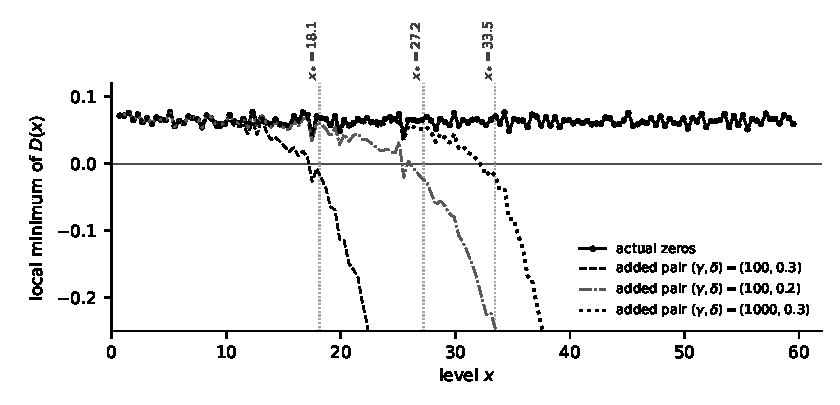
\includegraphics[width=0.8\textwidth]{fig/yo_off.pdf}
\caption{The least value of $D$ over windows of length $0.4$ on $[0,60]$, for the actual zeros (solid, the first $1700$ zeros with the smooth tail; the least window minimum is $0.0427$, in the window centred at $x=25.5$) and with one hypothetical off line pair added at height $\gamma$ and displacement $\delta$, $(\gamma,\delta)=(100,0.3)$ (dashed), $(100,0.2)$ (dash dotted) and $(1000,0.3)$ (dotted). Vertical dotted lines mark the predicted levels $x_*=18.1$, $27.2$ and $33.5$ of Remark~\ref{yo:rem:scale}. Script \texttt{yo\_tent.py}.}
\label{yo:fig:off}
\end{figure}

Table~\ref{yo:tab:D} compares the two sides of Proposition~\ref{yo:prop:tent}. The prime side is (c) with the exact $\Lambda(n)$. The zero side is $\sum_{\gamma>0}8\sin^2(\gamma x/2)/\gamma^2$ over the first $1500$ zeros (to height $1980.91$) plus the mean tail $2(\log(T/2\pi)+1)/(\pi T)$ at $T=\gamma_{1500}$. The two sides agree to $3.6\times10^{-6}$ at every level of the table except $x=\log2$ and $x=\log5$, where they differ by $1.6\times10^{-4}$ and $2.3\times10^{-4}$. These are the corners of the prime side at $x=\log n$, where its slope drops by $2\Lambda(n)/\sqrt n$, which a zero sum cut at $T$ and completed by a mean tail cannot follow: by Landau's formula \cite{Landau11} for $\sum_{0<\gamma\le T}n^{i\gamma}$ the zeros above $T$ contribute $2\Lambda(n)/(\pi\sqrt n\,T)$ at $x=\log n$, which is $1.575\times10^{-4}$ and $2.313\times10^{-4}$ at $T=\gamma_{1500}$, and with it the two corner rows agree to $1.3\times10^{-6}$. The last two columns agree to $10^{-29}$ in every row (eight decimals are printed). The values come from the script \texttt{yo\_explicit.py} (\texttt{code/\allowbreak README.md}).

\begin{table}[ht]
\centering\small
\begin{tabular}{rrrrr}
\toprule
$x$ & prime side & zero side & $V_1(\Delta_x)$ by (c) & by (d)\\
\midrule
0.2 & 0.1089996 & 0.1089981 & 0.25787887 & 0.25787887\\
0.5 & 0.0803252 & 0.0803270 & 0.15008051 & 0.15008051\\
$\log2$ & 0.1271112 & 0.1269547 & $-0.04998528$ & $-0.04998528$\\
1.0 & 0.0880146 & 0.0880147 & $-0.50847597$ & $-0.50847597$\\
1.5 & 0.0898189 & 0.0898186 & $-1.52909231$ & $-1.52909231$\\
$\log5$ & 0.1343264 & 0.1340964 & $-1.78866457$ & $-1.78866457$\\
2.0 & 0.1066822 & 0.1066850 & $-2.80144646$ & $-2.80144646$\\
3.0 & 0.0794186 & 0.0794176 & $-5.86891443$ & $-5.86891443$\\
4.0 & 0.0702819 & 0.0702855 & $-9.39384635$ & $-9.39384635$\\
6.0 & 0.0962464 & 0.0962437 & $-17.16435327$ & $-17.16435327$\\
\bottomrule
\end{tabular}
\caption{The tent value $D(x)$ from the primes (Proposition~\ref{yo:prop:tent}(c)) and from the zeros, and $V_1(\Delta_x)$ by the closed form (c) and by the residue series (d). The rows $x=\log2$ and $x=\log5$ differ by Landau's term, see the text.}
\label{yo:tab:D}
\end{table}

\section[The sine squared lemma off the diagonal]{The sine squared lemma off the diagonal: Yoshida's matrix is a L\"owner matrix}\label{yo:sec:lowner}

Recall Yoshida's basis $\chi_n=(2a)^{-1/2}e^{\pi iny/a}1_{[-a,a]}$ of $K(a)$ (Section~\ref{yo:sec:yoshida}, \cite{Yoshida92}), and write $\nu_n=\pi n/a$. The Fourier transform of the basis vector is
\[
\widehat{\chi_n}(t)=(2a)^{-1/2}\int_{-a}^ae^{i(t+\nu_n)y}\,dy=(2a)^{-1/2}\,\frac{2(-1)^n\sin(at)}{t+\nu_n},
\]
because $\sin(a(t+\nu_n))=(-1)^n\sin(at)$. Every basis vector carries the same factor $\sin(at)$; only the pole moves. The L\"owner matrix of a function $g$ on the nodes $\nu_n$ has the entries $(g(\nu_n)-g(\nu_m))/(\nu_n-\nu_m)$ off the diagonal and $g'(\nu_n)$ on it, and a Pick function is a function holomorphic on the upper half plane with nonnegative imaginary part there.

\begin{theorem}\label{yo:thm:lowner}
\begin{itemize}
\item[(i)] Unconditionally,
\[
\langle\chi_n,\chi_m\rangle=(-1)^{n+m}\,\frac2a\sum_\rho\frac{\sin^2(a\gamma_\rho)}{(\gamma_\rho+\nu_n)(\gamma_\rho+\nu_m)},
\]
an absolutely convergent series.
\item[(ii)] Let $g_a(\nu)=\sum_\rho\sin^2(a\gamma_\rho)/(\gamma_\rho-\nu)$, the sum over all zeros taken in symmetric pairs; unconditionally it is an odd meromorphic function of $\nu$. Then for $n\ne m$
\[
\langle\chi_n,\chi_m\rangle=(-1)^{n+m}\,\frac2a\,\frac{g_a(\nu_n)-g_a(\nu_m)}{\nu_n-\nu_m},\qquad \langle\chi_n,\chi_n\rangle=\frac2a\,g_a'(\nu_n),
\]
so Yoshida's matrix is, up to the sign change $\operatorname{diag}((-1)^n)$, $\frac2a$ times the L\"owner matrix of $g_a$ on the lattice $\frac\pi a\mathbb Z$.
\item[(iii)] Under RH, with the weighted Thorin measure $U_a^\sharp(dt)=2\sin^2(a\sqrt t)\,U(dt)\ge0$ and its Stieltjes transform $\mathcal S_a(s)=\int U_a^\sharp(dt)/(t+s)$,
\[
\begin{gathered}
g_a(\nu)=\nu\,\mathcal S_a(-\nu^2),\\
\langle\chi_n,\chi_m\rangle=(-1)^{n+m}\frac2a\int\frac{2\sin^2(a\sqrt t)\,(t+\nu_n\nu_m)}{(t-\nu_n^2)(t-\nu_m^2)}\,U(dt),
\end{gathered}
\]
and $g_a$ is an odd Pick function. By the elementary half of L\"owner's theorem every finite Yoshida matrix is then positive semidefinite, for every $a$.
\item[(iv)] For each fixed $a>0$, RH holds if and only if $g_a$ is a Pick function.
\end{itemize}
\end{theorem}

\begin{proof}
(i) $F=\chi_n*\widetilde{\chi_m}$ has $\widehat F(t)=\widehat{\chi_n}(t)\overline{\widehat{\chi_m}(\overline t)}=(-1)^{n+m}\frac2a\sin^2(at)/((t+\nu_n)(t+\nu_m))$, entire because $\sin^2(at)$ vanishes at $-\nu_n$ and $-\nu_m$. It is $O(t^{-2})$ in every strip, and $F$ is continuous, piecewise smooth and compactly supported, so \eqref{yo:EF} applies to it as it does to the tent (proof of Proposition~\ref{yo:prop:tent}(c)). Sum $\widehat F(\gamma_\rho)$.

(ii) Replace $\gamma_\rho$ by $-\gamma_\rho$ (the zero set is symmetric), then use $\frac1{(\gamma-\nu_n)(\gamma-\nu_m)}=\frac1{\nu_n-\nu_m}\bigl(\frac1{\gamma-\nu_n}-\frac1{\gamma-\nu_m}\bigr)$; the diagonal is the limit. The series of $g_a$ converges in symmetric pairs, since the pair $\pm\gamma_\rho$ contributes $2\nu\sin^2(a\gamma_\rho)/(\gamma_\rho^2-\nu^2)=O(|\nu|\,|\gamma_\rho|^{-2})$, and $g_a(-\nu)=-g_a(\nu)$ because the zero set is symmetric. A zero with $\gamma_\rho=\nu_n$ contributes nothing at the lattice, since $\sin^2(a\gamma_\rho)=0$.

(iii) Under RH group $\pm\gamma$: $\sin^2(a\gamma)\bigl(\frac1{\gamma-\nu}-\frac1{\gamma+\nu}\bigr)=\frac{2\nu\sin^2(a\gamma)}{\gamma^2-\nu^2}$, and with $t=\gamma^2$ this is $\nu\int U_a^\sharp(dt)/(t-\nu^2)$. In the same way the pair $\pm\gamma$ in (i) gives $2\sin^2(a\gamma)(\gamma^2+\nu_n\nu_m)/((\gamma^2-\nu_n^2)(\gamma^2-\nu_m^2))$, which is the second formula. Each atom $\nu/(t-\nu^2)$ has imaginary part $\Im\nu\,(t+|\nu|^2)/|t-\nu^2|^2>0$ for $\Im\nu>0$, so $g_a$ is a Pick function. For a Pick function $g$ and real nodes $\nu_1,\dots,\nu_N$, the matrix $[(g(\nu_i)-g(\nu_j))/(\nu_i-\nu_j)]$ is positive semidefinite, which is L\"owner's easy direction \cite{Lowner34,Donoghue74}.

(iv) If RH fails, an off line pair gives the nonreal ordinates $\pm\gamma\pm i\delta$, two of them in the upper half plane, where $g_a$ has a pole with residue $-m\sin^2(a\gamma_\rho)$, $m$ the multiplicity. This residue is nonzero because $\sin$ vanishes only on the real axis, and a Pick function is holomorphic in the upper half plane. The converse is (iii).
\end{proof}

The mechanism of the theorem is that of the rigidity of the clock, Proposition~\ref{prop:rigid}: there $G'/G$ is the Stieltjes transform of $U$, holomorphic off the negative real axis exactly when every zero is on the line, and $\mathcal S_a$ is the same transform with the atoms weighted by $2\sin^2(a\gamma)$, sampled on the cut at the squared modal frequencies $\nu_n^2$ and differenced.

Numerically, the prime side of $\langle\chi_n,\chi_m\rangle$, computed from \eqref{yo:EF} and \eqref{yo:V1} by Gauss Legendre quadrature, gives the coefficient $\langle\chi_0,\chi_0\rangle=0.18338$ of Yoshida's matrix at $a=\frac12\log2$, and at $a=1$ it matches part (i) summed over the first $1500$ zeros, entry by entry, up to the zero tail. The tail of the smooth count from $T=1982.0$ accounts for the difference up to $9\times10^{-7}$ (\texttt{yo\_explicit.py}, \texttt{code/\allowbreak README.md}).
